% !TEX root = ../../../main.tex
% 来源：中学数学实验教材·第一册（代数）
% 章节：因式分解与余式定理 / 辗转相除法
% 原始文件：5.tex，行 2763-2788
% 类型：tikz
% ---
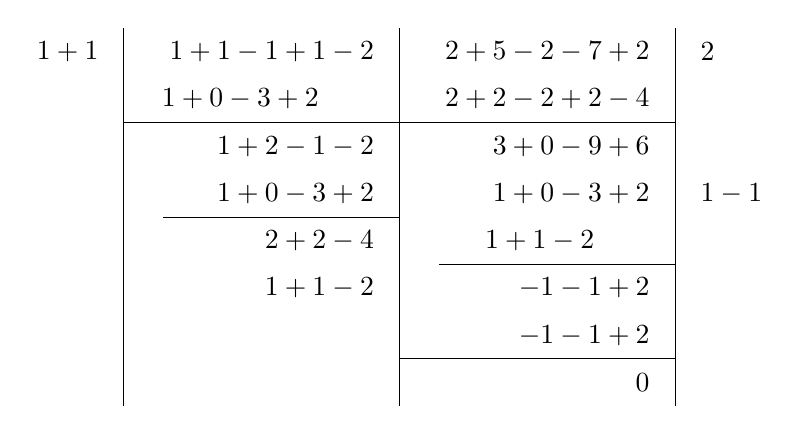
\begin{tikzpicture}[yscale=.6]
\foreach \y/\ytext in {6/1+1-1+1-2   ,5/1+0-3+2\qquad  ,4/1+2-1-2   ,3/ 1+0-3+2  , 2/2+2-4 ,1/\boxed{1+1-2} }
{
    \node at (.3,\y)[left]{$\ytext$};
}

\foreach \y/\ytext in {6/2+5-2-7+2  ,5/2+2-2+2-4  ,4/ 3+0-9+6 , 3/ 1+0-3+2  , 2/1+1-2\qquad  , 1/-1-1+2, 0/-1-1+2, -1/0}
{
    \node at (3.8,\y)[left]{$\ytext$};
}

\foreach \x in {-3,0.5,4}
{
    \draw(\x,6.5)--(\x, -1.5);
}

\draw (-3,4.5)--(4,4.5);

\draw (-2.5,2.5)--(.5,2.5);
\draw (.5,-.5)--(4,-.5);
\draw (1,1.5)--(4,1.5);

 \node at (4.2,6)[right]{$2$};
 \node at (4.2,3)[right]{$1-1$};
 \node at (-3.2,6)[left] {$1+1$};
\end{tikzpicture}
